% 
% Licensed under Creative Commons Attribution Share Alike 4.0 International
% SPDX-License-Identifier: CC-BY-SA-4.0
% 
\documentclass[
portrait,a0paper
% landscape,
%draft
]{baposter}
%
% load packages
% already loaded some useful packages for figures, tables and layout
% not all are needed to run this minimal example
\usepackage{graphicx}
\usepackage[percent]{overpic}
\usepackage[detect-weight]{siunitx}
\usepackage{tabto}
\usepackage{booktabs}
\usepackage{amsmath}
\usepackage{float}
\usepackage{multirow}
\usepackage{url}
\usepackage{enumitem}
\usepackage{qrcode}
\usepackage[backend=biber]{biblatex}
\addbibresource{main.bib}
\usepackage{multicol}
\usepackage{listings}
\usepackage{textcomp}
\usepackage{qrcode}
% add additional packages you need here
%
% for now usig bibitem, but if you want ...
%\usepackage[backend=biber]{biblatex} 
%
% customizing 
\newlength{\mytextsize}
\newcommand\e{\cdot 10^}
\setlength{\unitlength}{1.0cm}
%
% define ASF orange
\definecolor{bkgndColor}{cmyk}{.79,0,.62,.28} 
% fonts
\usepackage[scaled]{helvet}
\renewcommand*\familydefault{\sfdefault}
%
%
%##################################################################################
\begin{document}
%##################################################################################
\begin{poster}
{
  % options
  grid=false,%true,
  background=plain,
  bgColorOne=white,
  columns=6, % for flexibility changing 2/3 columns with columnspan
  eyecatcher=false,
  borderColor=bkgndColor,
  headerColorOne=bkgndColor, %white,
  headershade=plain,
  %headerColorTwo=white,
  headerborder=open,
  % for rectangular boxes change the next two options, rectangular header will cause left aligning of box title 
  textborder=rounded, %rectangle,
  headershape=rounded, %rectangle,
  headerfont=\bf\Large,
  boxshade=none,
  headerFontColor=white
}
{
  %eyecatcher ...
}
{
  %poster title
  % first put graphics for header
  \hspace*{-0.5mm}
  \begin{picture}(23.7, 2)
  \fboxsep0pt
  \put(-0.196, -0.6){\colorbox{bkgndColor}{\rule[96pt]{675.82pt}{0pt}}}
  \thicklines
  % minipage box for title and authors
  \put(2.55, 2.35){
    \begin{minipage}[t][96pt]{0.75\textwidth}
    % centering
    \begin{center}
    % Title
    % use \LARGE instead of \Huge for long titles, you might need to modify distances or number of lines
    % for one line title
    %\ \vspace{0.15cm}\\
    %\huge\bf\color{white}\selectfont Single Line Title \vspace{0.4cm}\\ 
    % for two line title
    \huge\bf\color{white}\selectfont A Wildcard Matcher Search Strategy \\ 
    %\huge\bf\selectfont  \vspace{0.15cm} \\ 
    % Authors, main author first will be underlined, you might need to modify distances or number of lines
    % three lines
    \small\underline{Claude N. Warren, Jr.} \\
    %\small C.\ Author, Institute \\
    %\small D.\ Author, Institute
    % two lines
    \vspace{0.5cm}
    \color{white}\small Text licensed under Creative Commons CC-BY-SA-4.0 \\
    \color{white}\small Code licensed under Apache License 2.0 \\
  


    %\small\underline{Main Author}, B.\ Author, CERN, Geneva, Switzerland \\
    %\small C.\ Author, Institute \\
    \end{center} 
  \end{minipage}}
  %  
  % cern logo
  % left:
  %\put(0.32,-0.24){\includegraphics[height=75pt]{logos/LogoOutline-White.eps}}
  % right:
  %\put(20.52,-0.24){\includegraphics[height=75pt]{logos/LogoOutline-White.eps}}
  %% DO NOT FORGET to replace QR code link and Poster ID !
  % % poster id + qr code, for example at IPAC
  % Modify links!!!
  % left
  \put(0.18,1.1){\color{white}\qrcode[hyperlink,height=.08\textwidth]{https://github.com/Claudenw/BloomTextFilter}}
  
  % right
  %\put(21.02,-0.25){\large\bf\color{white}Poster ID}
  %\put(21,1.1){\color{white}\qrcode[hyperlink,height=.08\textwidth]{https://gitlab.cern.ch/mkoopman/templates}}
  \end{picture} 
}
{
	%poster authors, already in title
}
{
	%logo, already in title
}
%
% three part footnote box with references, logos, contact infos
%

\headerbox{}{headershape=rectangle, name=foottext, column=0, span=6, above=bottom, textborder=none, borderColor=bkgndColor,  boxheaderheight=1pt} {
    \printbibliography[title={\textbf{\small\color{bkgndColor}KEY REFERENCES}\footnotesize\\}]
}

%
% and now the standard boxes on the poster
% choose between 2 or 3 column layout here!
% for 2 column layout use column=0 and column=3, respectively (always span=3)
% for 3 column layout use column=0, column=2 and column=4, respectively (always span=2)
% or go with 6 columns and column span ... 
%
% in the following is here a simple example for two column layout with
% three boxes on the left: motivation, left box 1, left box 2 and
% two boxes on the right: large right box, summary
%
\headerbox{Motivation}{name=motivation, column=0, row=0, span=3}{

   There are times when a single string exemplar must be checked against a number of wildcard patterns to find the best match.  This poster presents a strategy for rapidly selecting patterns to check and selecting the best fit among the matches. \\
   
   An application for such a strategy is the application of Access Control Lists constraints on value to determine if a user has access. \\

   The solution presented here assumes that the more similar the wildcard is to the pattern the higher precedence it has in terms of evaluation.
}
%
%
\headerbox{Background}{name=bkgrnd, span=3, below=motivation, column=0}{
  Let's explore the ACL use case and make the following assumptions: 
  \begin{itemize}
      \item The wildcard patterns use asterisks (*) to denote one or more characters.
      \item The wildcard is implemented as a regular expression replacing the asterisk with the regular expression '.*' to match multiple characters.
  \end{itemize}

  The naive algorithm for finding the set of matching patterns for a single target is:
  \begin{itemize}
      \item Create a list of patterns ordered by the number of non-wildcard characters.
      \item Iterate through the list evaluating each one if a match is found add the pattern to the list of potential solutions.  Stop when the number of non-wildcard characters exceeds the number of characters in the length of the target.
      \item Check each potential solution using a standard measure of text similarity to find the closest match.
  \end{itemize}

}
%
%
\headerbox{Extracting Sequences}{name=seq, span=3, below=bkgrnd, above=foottext, column=0}{
  This strategy will exploit the work on sequence characterization in bioinformatics\cite{solomon2016fast}.  We begin by converting each wildcard pattern set of Hashers\cite{website:Hasher} that represents each pair of characters in the text by:
    \item ~~Breaking the text into chunks whenever a non character or digit is found.
    \item ~~Remove any chunks that have fewer than 2 characters. 
    \item ~~Remove any duplicate chunks. 
    \item ~~For each $chunk$ 
    \item ~~~~For (int i=0,i<$chunk$.length-2; i++) 
    \item ~~~~~~token = $chunk$.substring(i,2) 
    \item ~~~~~~long[] hash = MurmurHash3($token$) 
    \item ~~~~~~hashes.add(new EnhancedDoubleHasher(hash[0], hash[1])) 
    \item ~~return hashes  
  
  The hashes can then be used to create a Bloom\cite{bloom1970space} filter using the Apache Commons Collections\textregistered~library.\\

  The Bloom filters for the wildcard patterns will have fewer sequences than the patterns they match.  This means that we can check if the target Bloom filter contains the wildcard Bloom filter and if so evaluate the pattern for a match.
}
%
%
\headerbox{Selecting The Match}{name=select, span=3, row=0, column=3}{
  The patterns returned from Extracting Sequences should be compared using a standard measure of similarity like Levenshtein Distance\cite{website:LevenshteinDistance} to determine the distance from the target to the pattern.  Patterns with smaller distances should be selected over patterns with greater distances.  For patterns with the same distances, longer patterns (more specificity) should be selected over shorter patterns. \\

  Finally, the patterns should be tested against the target in the order determined above.  The fist matching target is the best fit.
}		
%
%
\headerbox{Experimental Results}{name=summary, span=3, below=select, above=foottext, column=3}{
 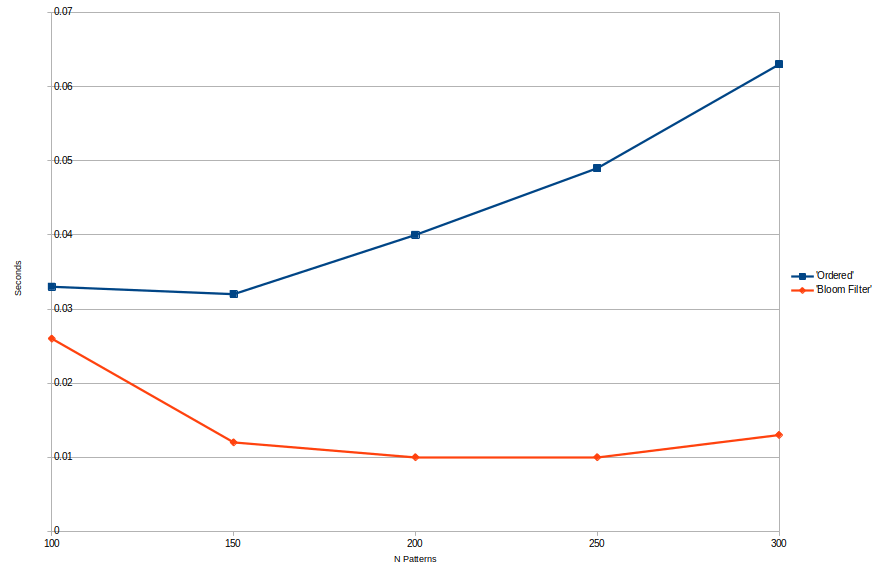
\includegraphics[scale=.35]{images/graph.png}
 The graph shows a run of the test code\cite{website:Poster} with 100 to 300 patterns. The experiment selected 50 words at random and generates a number of phrases from those words.  Two to four words are combined with hyphens '-' to create the number of phrases.  The phrases are selected at random, and one or more hyphen separated parts are replaced with asterisks '*' to create the patterns. The table below shows the number of phrases associated with the number of patterns.  Each phrase is then tested against the patterns finding the best fit as described in the Motivation section above.  The results show that the Bloom filter based search out performs the naive brute force method even for as few as 100 patterns.
\begin{center}
 \begin{tabular}{ || r | r ||}
   \hline
   Patterns & Phrases  \\
   \hline
    100 & 500 \\
   \hline
     150 & 750 \\
   \hline
    200 & 1000 \\
   \hline
    250 & 1250 \\
   \hline
    300 & 1500 \\ 
  \hline
 \end{tabular}
\end{center}
  The Bloom filters in the experiment are based on the number of 2-character chunks that were developed for the longest phrase.  The maximum bloom filter size was 85 bytes.  This means that the solution requires 85 bytes per pattern to implement.
}
%
%
\end{poster}
\end{document}